\subsection{Reverse Engineering}

\begin{frame}
    \frametitle{Reverse engineering}
    Uno dei punti di forza di MIFARE è il bassissimo costo di produzione.

    Il circuito che si occupa della logica dell'integrato è composto da circa 400 porte NAND (equivalenti)~\cite{nohl2008reverse}

    \begin{figure}
        \centering
        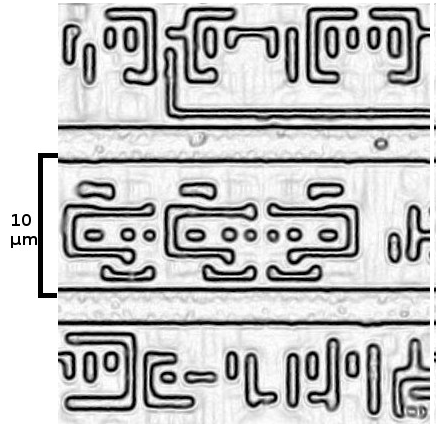
\includegraphics[width=0.2\textwidth]{ReverseEngeneering.png}
        \caption{Immagine tratta da~\cite{nohl2008reverse} presa da un microscopio ottico (500x) e processata con filtri di edge detection}
        \label{fig:reverse-engeneering}
    \end{figure}
\end{frame}

\begin{frame}
    \frametitle{Reverse engineering}
    Grazie alle ricerche e allo studio degli integrati (fig~\ref{fig:reverse-engeneering}), è stato possibile dedurre il circuito logico utilizzato
    al fine di implementare la crittografia della fase di autenticazione.

    Il circuito si presenta come segue:
    \begin{figure}
        \centering
        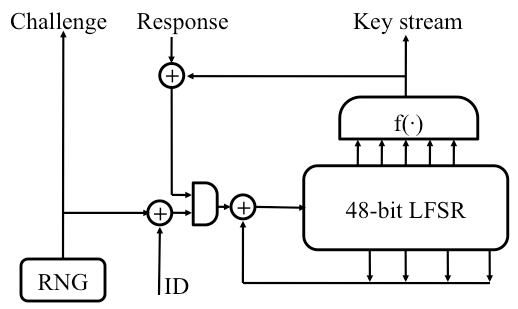
\includegraphics[width=0.3\textwidth]{authLogic.png}
        \caption{Circuito logico ricavato dal reverse engineering del tag}
        \label{fig:reverse-engeneering-circuit}
    \end{figure}
\end{frame}
\note{
    Dal seguente schema è possibile ricavare il funzionamento completo del processo di autenticazione a un blocco.
    In particolare è possibile definire con certezza le funzioni 
    \[cipherInit(key, uid, n_t) = f(key)\]
    Si noti che la funzione configura i parametri \(uid\) e \(n_t\) proveniente dal RNG.
    \[cipher(n_r) = f(next\_iteration())\]
    dove \(n_r\) viene impostato precedentemente all'iterazione.

    Il procedimento permette così di configurare in modo identico i due stream cipher per garantire di avere due stream di chiavi uguali per cifrare la comunicazione.
}

\begin{frame}
    \frametitle{Struttura matematica i}
    Indichiamo \(var_i\) l'i-esimo bit della variabile var \\
    Indichiamo \(bits(num)\) la funzione che ritorna il numero di bit che compongono \(num\)
    Indichiamo \(L(LFSR)\) il risultato della funzione di feedback del LFSR~\cite{garcia2008dismantling}

    \pause
    Definiamo la funzione \(set(key, s)\) che imposta il valore di LFSR allo stato s con il valore \(key\)
    \[set(key, s) = LFSR_i := key_i \forall i \in [0, bits(num))\]

    \pause
    Definiamo quindi la funzione \(next(bit, s)\) la funzione che effettua l'iterazione sullo LFSR
    \[next(bit, s) = set(LFSR[47..1] || L(LFSR) \oplus bit, s)\]
\end{frame}

\begin{frame}
    \frametitle{Struttura matematica ii}
    Indichiamo la funzione \(f(LFSR, s)\) la filter function (si veda \cite{garcia2008dismantling}) che ritorna il valore del keystream allo stato s

    Indichiamo la funzione \(rnd()\) la funzione che genera un numero casuale

    \pause
    Definiamo \(push(value, s)\) la funzione che aggiorna lo LFSR con il valore \(value\)
    \[push(value, s) = next(value_i, s) \forall i \in [0, bits(value))\]

    \pause
    Indichiamo \(suc^n(seed)\) la funzione che ottiene i successivi 32 bit dal RNG~\cite{secRFIDMutualAuth}

    \pause
    Definiamo infine \(ks(s)\) la funzione che ritorna la chiave corrispondente allo stato s
    \[ks(s) = f(LFSR, s)\]
\end{frame}

\begin{frame}
    \frametitle{Struttura matematica iii}
    Definiamo ora il processo di autenticazione di un blocco, dove \(skey\) è la chiave condivisa ottenuta dalla memoria del tag e con la quale il lettore si vuole autenticare.
\end{frame}

\begin{frame}
    \frametitle{Struttura matematica iv}
    \begin{columns}
        \column{0.5\textwidth}
        \centering{\textbf{TAG}}
        \column{0.5\textwidth}
        \centering{\textbf{READER}}
    \end{columns}
    \begin{columns}
        \column{0.5\textwidth}
            \(n_t = rnd()\)\\ \pause
            \(s = push(n_t \oplus uuid, set(skey, s))\)\\ \pause
            \(send(n_t)\)\pause
        \column{0.5\textwidth}
    \end{columns}
    \begin{columns}
        \column{0.5\textwidth}
        \column{0.5\textwidth}
            \(n_t = recv()\)\\\pause
           \(s = push(n_t \oplus uuid, set(skey, s))\)\\\pause
            \(n_r = rnd()\)\\\pause
            \(send(n_r \oplus ks(s))\)\\\pause
            \(s = push(n_r, s)\)\\\pause
            \(send(suc^2(n_t) \oplus ks(s))\)
    \end{columns}
\end{frame}

\begin{frame}
    \frametitle{Struttura matematica v}
    \begin{columns}
        \column{0.5\textwidth}
            \(n_r = recv() \oplus ks(s)\)\\\pause
            \(s = push(n_r, s)\)\\\pause
            \(assert(suc^2(n_t) == recv() \oplus ks(s))\)\\\pause
            \(s = push(n_r, s)\)\\\pause
            \(send(suc^3(n_t) \oplus ks(s))\)\pause
        \column{0.5\textwidth}
   \end{columns}
    \begin{columns}
        \column{0.5\textwidth}
        \column{0.5\textwidth}
            \(a_r = recv() \oplus ks(s)\) \pause
            \(assert(suc^3(n_t) == a_r)\)
    \end{columns}
\end{frame}

\subsubsection{Filter Function}
\begin{frame}
    \frametitle{Analisi della funzione di filtraggio}\label{sec:filter-fn}
    È possibile controllare interamente lo stato del LFSR grazie al fatto che tutti i parametri sono visibili.\pause

    Essendo il protocollo di comunicazione documentato, è possibile inviare al lettore/tag dati personalizzati.\pause

    È quindi possibile inviare al lettore chiave, UUID e nonce pari sempre a 0 (o a un valore noto) in modo da controllare lo stato $\alpha$ dell'LFSR \pause

    Inoltre è possibile mantenere $n_r$ costante riavviando il lettore ogni volta
\end{frame}

\begin{frame}
    \frametitle{Analisi della funzione di filtraggio}
    È possibile quindi dedurre informazioni sulla funzione $f$ variando di un bit lo stato $\alpha$.\pause

    Se $f(\alpha) \neq f(\alpha')$ allora il bit modificato farà parte degli input della funzione $f$
    Altrimenti non è possibile dedurlo con certezza\pause

    Tramite inferenza statistica si può raggiungere una discreta certezza a riguardo
\end{frame}
\note{
    
}
\begin{frame}
    \frametitle{Analisi della funzione di filtraggio}
    Dopo una ricerca esaustiva si è giunti a ricavare la seguente funzione f
    \begin{figure}
        \centering
        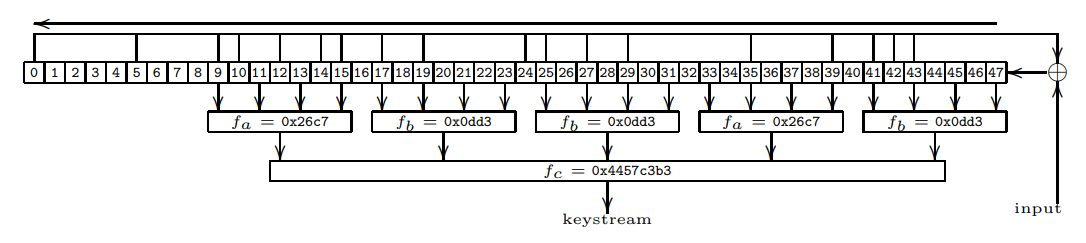
\includegraphics[width=0.9\textwidth]{crypto1.png}
        \caption{Risultato del reverse engineering e dei test\cite{garcia2008dismantling}}
        \label{fig:crypto1}
    \end{figure}
\end{frame}
\note{
    Si noti la grande somiglianza con lo stream chipher Hitag2.
    Questo cifrario è utilizzato solitamente nelle chiavi delle automobili dotate di verifica wireless del dispositivo tramite RFID (125kHz).

    Anche questo cifrario è stato dichiarato insicuro e vulnerabile.\cite{verdult2012gone}
    \begin{figure}
        \centering
        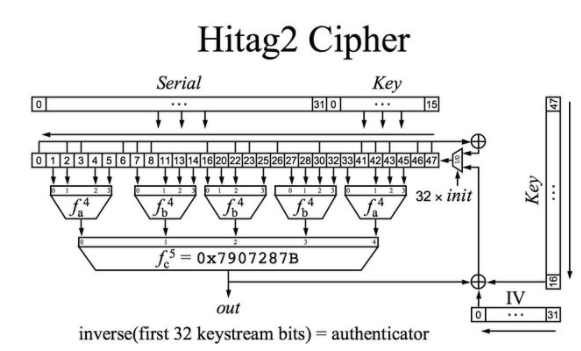
\includegraphics[width=.5\textwidth]{hitag2.png}
        \caption{Cifrario Hitag2}
    \end{figure}
}